\documentclass[10pt,a4paper]{article}

% ---------------------------------------------------------------------------
% Shared knowledge in agent teams, explained in plain language.
% Companion to docs/follow-up-study-DS-A2A.tex (the research paper) and to
% docs/AgentM2M-explained.tex (the walkthrough of the base system).
%
% Every number in this document comes from the experiments in
% evaluation/results/follow-up-study/ (csv/ and tables/): 3 seeds of the 7B
% model on 8 DevBench repositories, 2 seeds of the 27B model on 4 of them,
% finished on 2026-10-07. Every listing marked "engine" is real output of the
% prototype (evaluation/harness/chakin_context_walkthrough.py).
% ---------------------------------------------------------------------------

\usepackage[T1]{fontenc}
\usepackage[utf8]{inputenc}
\usepackage{lmodern}
\usepackage[margin=2.3cm]{geometry}
\usepackage{amsmath,amssymb}
\usepackage{booktabs,array,tabularx,multirow}
\usepackage{xcolor}
\usepackage{enumitem}
\usepackage{listings}
\usepackage{graphicx}
\graphicspath{{../evaluation/results/follow-up-study/figures/}}
\usepackage{tikz}
\usetikzlibrary{arrows.meta,positioning,shapes.geometric,fit,calc}
\usepackage[strings]{underscore}
\usepackage[hidelinks]{hyperref}
\usepackage{cleveref}

\newcommand{\tool}{\textsc{AgentM2M}}
\newcommand{\code}[1]{\texttt{#1}}
\newcommand{\file}[1]{\texttt{#1}}

\definecolor{rawbg}{RGB}{255,248,230}
\definecolor{modelbg}{RGB}{235,244,255}
\definecolor{enginebg}{RGB}{236,250,238}
\definecolor{llmbg}{RGB}{248,238,252}
\definecolor{noteboxbg}{RGB}{245,245,245}

\lstset{frame=single, basicstyle=\ttfamily\footnotesize, breaklines=true,
        breakatwhitespace=false, columns=fullflexible, keepspaces=true,
        showstringspaces=false, numbers=none, upquote=true,
        captionpos=t, aboveskip=6pt, belowskip=6pt}
\lstdefinestyle{raw}{backgroundcolor=\color{rawbg}}
\lstdefinestyle{model}{backgroundcolor=\color{modelbg}}
\lstdefinestyle{engine}{backgroundcolor=\color{enginebg}}
\lstdefinestyle{llm}{backgroundcolor=\color{llmbg}}
\crefname{lstlisting}{Listing}{Listings}
\Crefname{lstlisting}{Listing}{Listings}

% a framed one-line takeaway
\newcommand{\takeaway}[1]{\par\medskip\noindent\fcolorbox{black!35}{noteboxbg}{%
  \parbox{0.95\linewidth}{\small\textbf{In one sentence.} #1}}\par\medskip}
% the "analogy" marker
\newcommand{\analogy}[1]{\par\smallskip\noindent\textit{Think of it like this: #1}\par\smallskip}

\title{Shared Knowledge in Agent Teams, Explained\\[2pt]
\large A plain-language walkthrough, with the results of our experiments}
\author{Companion document to ``Selective Knowledge Pinning for LLM Agent Teams''}
\date{}

\begin{document}
\maketitle

\begin{abstract}
A team of AI agents that builds software shares two things. The first is \emph{work}: the
requirements, design, code and tests that move from one agent to the next. The second is
\emph{knowledge}: a security finding, a design decision, a rule such as ``never write outside the
download folder''. Work already has a tidy way to travel in our system. Knowledge did not: teams
copy it into prompts by hand, so nobody can say which piece of code was written under which version
of a finding, a changed finding sets off either too much redoing or whatever a person remembers to
redo, and nobody can watch the team without reading its chat. This document explains, in simple
terms and step by step, the three things we added: a \emph{shared notebook} that agents read under
clear rules; a way to \emph{ask who used which page}; and a \emph{logbook} that records everything
the team does without ever changing it. It then shows what happened when we tried all of this
on 8 real software projects with 2 AI models, 128 team runs and 648 deliberately injected failures.
The short version: the notebook costs about as much as an expert who keeps a hand-written routing
table (about 17\% more tokens, the same number of AI calls), and about 3 times less than the
careless way of copying notes into every prompt. It also does the bookkeeping on its own, and the
logbook never changed a single outcome. We also show what it cannot do: it does not know whether a
note is true.
\end{abstract}

\tableofcontents

% ===========================================================================
\section{How to read this document}\label{sec:read}
% ===========================================================================

This document assumes no background in model-driven engineering, hashing or Nostr. Every technical
word is explained the first time it appears, and \Cref{sec:glossary} collects them. It has two kinds
of content.

\begin{itemize}[leftmargin=*]
\item \textbf{Explanations} (Sections~\ref{sec:problem}--\ref{sec:ideas}): what problem we are solving,
      the three ideas, and how each one works, with small examples. Real output from the prototype is shown
      in colour-coded boxes.
\item \textbf{Evidence} (Sections~\ref{sec:experiment}--\ref{sec:results} and \ref{sec:limits}): how we tested the
      ideas, the numbers we got, and, just as important, where the ideas fall short.
\end{itemize}

\begin{center}
\small
\begin{tabular}{@{}l p{11.5cm}@{}}
\toprule
\colorbox{rawbg}{\strut\ Raw input\ } & Something a person or a benchmark provides: a rule file, a request. \\
\colorbox{modelbg}{\strut\ Model\ } & A rule, a note or a record as the system holds it. \\
\colorbox{llmbg}{\strut\ LLM\ } & A prompt that is sent to an AI model. \\
\colorbox{enginebg}{\strut\ Engine\ } & Deterministic output of the system: fingerprints, logs, events, query answers. \\
\bottomrule
\end{tabular}
\end{center}

\paragraph{The whole idea in five sentences.}
(1)~Agents sometimes need to share \emph{knowledge}, not just hand over finished work.
(2)~We keep that knowledge in a shared notebook where every note has an author, a version and an
access list.
(3)~When an agent does a job, we record exactly which notes it read, and we mix a fingerprint of those
notes into the job's fingerprint.
(4)~So when a note changes, the system can tell, without anyone's memory, which jobs must be redone and
which are untouched, and it can answer ``what did this note influence?''.
(5)~Everything that happens is written to a logbook that cannot change the outcome, and the logbook can
optionally be copied, signed, to other machines.

\paragraph{What we ran.}
\Cref{tab:scope} shows the size of the experiment. All numbers in the rest of this document come from it.

\begin{table}[h]
\centering\small
\caption{What was run. A ``run'' is one team of agents building one repository once under one way of sharing
knowledge, followed by five changes to the shared knowledge.}
\label{tab:scope}
\begin{tabular}{@{}lll@{}}
\toprule
 & 7B model (\code{qwen2.5-coder:7b}) & 27B model (\code{qwen3.8:27b}) \\
\midrule
Software projects (DevBench, Python) & 8 & 4 (the smaller ones) \\
Repetitions with different random seeds & 3 & 2 \\
Ways of sharing knowledge compared & 4 & 4 \\
Runs & 96 & 32 \\
\midrule
Total runs & \multicolumn{2}{p{7.5cm}}{128, with no run failing} \\
Replays for the logbook tests & \multicolumn{2}{p{7.5cm}}{32 (one per project, model and seed)} \\
Failures injected on purpose & \multicolumn{2}{p{7.5cm}}{648 (576 in the four main families, 40 probes of known limits, 32 harmless controls)} \\
\bottomrule
\end{tabular}
\end{table}

% ===========================================================================
\section{The problem, in everyday terms}\label{sec:problem}
% ===========================================================================

\subsection{An office with four people and one pinned note}

Picture a small software office. The \emph{Analyst} writes requirements. The \emph{Architect} turns them
into a design. The \emph{Developer} writes code for each function in the design. The \emph{Tester} writes
checks for each requirement. Each person is an AI agent. A fifth person, the \emph{Security Reviewer}, joins
and writes down two findings:

\begin{lstlisting}[style=raw, caption={The security reviewer's findings for the \code{chakin} word-vector downloader (real text from the runs).}, label={lst:findings}]
finding-path : download(): `save_dir` comes from the caller. Resolve the target path
               and refuse to write outside save_dir (no '..', no absolute file names).
finding-tls  : download(): fetch vectors over https only; never fall back to http.
\end{lstlisting}

The Developer needs the first finding when writing \code{download()}. The Tester needs it when writing a check
for \code{download()}. Everyone else can ignore it. This is \emph{knowledge}: it belongs to no single stage of
the pipeline, and several people need it.

\subsection{Three things that go wrong}

\Cref{tab:problems} lists the three problems we address. Each one is a real problem of a team of people as
well; AI teams make them worse, because an AI agent re-reads everything it is given on every call and does not
remember who said what.

\begin{table}[h]
\centering\small
\caption{The three problems and what we added for each.}
\label{tab:problems}
\begin{tabularx}{\textwidth}{@{}l X X X@{}}
\toprule
 & What goes wrong & Everyday picture & What we added \\
\midrule
\textbf{K1} Untraceable & Nobody can say which piece of code was written under which version of a finding.
  & Someone pasted the rule into six messages. A week later the rule changes and nobody knows who has the old one.
  & Every note has a version, and every job records which notes it read (\emph{the pin}). A query returns the
    jobs behind a note. \\[3pt]
\textbf{K2} Redone by memory & After a change, you redo everything, or you rely on a routing table kept in
  someone's head. & ``The Tester needs the second rule but not the first'' lives only in the team lead's head.
  & The system compares fingerprints and redoes exactly the jobs whose notes changed. \\[3pt]
\textbf{K3} Unwatchable & Agents on different processes or machines leave no trail except chat.
  & You can see that things happened, not who knew what, or why something was redone.
  & A logbook of typed events, optionally copied, signed, to other machines. \\
\bottomrule
\end{tabularx}
\end{table}

\takeaway{The problem is not that agents lack knowledge; it is that nobody can \emph{see} where the knowledge
went, so changing it is either wasteful or risky.}

% ===========================================================================
\section{A two-minute refresher on the base system}\label{sec:base}
% ===========================================================================

The system we extend, \tool{} (explained in detail in \file{AgentM2M-explained.tex}), treats every
hand-off between agents as a small, well-defined translation, not as a chat. You only need four facts.

\begin{enumerate}[leftmargin=*]
\item \textbf{Each agent keeps its work in its own form.} The Analyst keeps user stories, the Architect keeps
      components and operations, the Developer keeps code edits, the Tester keeps test cases.
\item \textbf{A fixed engine does the structure; the AI only fills in values.} The engine decides \emph{which}
      code edits exist and what they are called. The AI writes only what a program cannot compute, such as the
      body of one function, and it sees only the pieces of input the job declares (its \emph{footprint}).
\item \textbf{Every finished value gets a fingerprint.} When the AI's answer passes its checks, the system
      stores the answer together with a fingerprint (a \emph{stamp}) of everything the AI was shown.
\item \textbf{A mismatch is a to-do.} If the input of a job later changes, its fingerprint no longer matches
      the stored one. The system calls this an \emph{obligation} and redoes only that job.
\end{enumerate}

\analogy{every finished dish in a restaurant has a card clipped to it that lists a fingerprint of the
ingredients used. When the supplier changes one ingredient, the kitchen compares fingerprints and only remakes
the dishes whose card no longer matches.}

What this base system lacked is a place for \emph{notes that no single dish owns}, such as ``no nuts in
anything''. That is what we added.

% ===========================================================================
\section{The three ideas, step by step}\label{sec:ideas}
% ===========================================================================

\subsection{Idea 1: a shared notebook that agents read under clear rules}

\subsubsection*{What is in the notebook}

The notebook is a list of \emph{contexts}. A context is a small collection of \emph{notes} (we call them
items) about one topic. \Cref{tab:notebook} shows the parts.

\begin{table}[h]
\centering\small
\caption{The parts of the shared notebook.}
\label{tab:notebook}
\begin{tabularx}{\textwidth}{@{}l X@{}}
\toprule
Part & Meaning \\
\midrule
Item (a note) & One fact with an id, a type (``security-finding''), the text, who wrote it, and where it came from.
  It is a fact, not a chat transcript. \\
Version (a snapshot) & Each change to a context makes a new, unchangeable version. Old versions stay readable. Each
  version has a fingerprint of its contents. Writing identical contents makes no new version. \\
Access list (the policy) & Who owns it, who may write, who may read, whether it stays on this machine or may be
  shared, and when it expires. \\
Pin & The record a finished job keeps: which context, which version, which notes it read. \\
\bottomrule
\end{tabularx}
\end{table}

The notebook enforces its own access list for everyone. A note is always credited to the agent that wrote it,
an update that is based on an out-of-date version is refused (it never silently overwrites someone else's
work), and a missing, expired or forbidden context gives the reader nothing at all.

\subsubsection*{How a job says which notes it needs}

In a rule, a job lists the notes it wants. It can ask for one page of the notebook or for the whole thing:

\begin{lstlisting}[style=model, caption={Two jobs. The Developer's code job reads one note; the Tester's job reads the whole context. (Real rule variants from the experiment.)}, label={lst:rule}]
body   <- @llm('Implement this operation ...', op.codeContext(),
               context = ['security-review#finding-code']),     -- one note
oracle <- @llm('Write a test oracle ...', c.text,
               context = ['security-review'])                   -- the whole context
\end{lstlisting}

When the job runs, the notes it was granted are added to the prompt in a clearly labelled, read-only section,
so the AI model can use them and so an auditor can see exactly what it was given:

\begin{lstlisting}[style=llm, caption={Part of a real prompt for the Developer's \code{download} job (the end of the prompt).}, label={lst:prompt}]
Authorized shared context (read-only collaboration knowledge; use it, do not invent more):
[context security-review v2 sha256:47d98089c005] -- Security review findings
- finding-path (security-finding, by SecurityReviewer): download(): `save_dir` comes from
  the caller. Resolve the target path and refuse to write outside save_dir ...
- finding-tls (security-finding, by SecurityReviewer): download(): fetch vectors over
  https only; never fall back to http.
\end{lstlisting}

\subsubsection*{The key trick: the fingerprint includes the notes}

This is the heart of the idea, and it is small. Before, a job's fingerprint covered \emph{only its input}. Now it
covers its input \emph{plus a fingerprint of exactly the notes it asked for}:
\[
\text{fingerprint of a job} \;=\; \text{fingerprint}\bigl(\text{its input},\ \text{fingerprint of the notes it reads}\bigr).
\]
A job that asks for no notes keeps exactly the old fingerprint, so existing teams are unaffected. After a job is
finished, the system keeps the pin and the three fingerprints that make it up:

\begin{lstlisting}[style=engine, caption={What the system stores for the finished \code{download} code job (real output). The ``effective'' fingerprint is the one compared later.}, label={lst:trace}]
"stamps":       { "body": "3e0a20f81349f199" },
"context_pins": { "body": [ { "context_id": "security-review", "version": 2,
                              "item_ids": [], "content_digest": "47d98089c005fd4f..." } ] },
"dependencies": { "body": { "source":    "71599f67c7a21b83",    <- its normal input
                            "context":   "00a4f03750fa6202",    <- the notes it read
                            "effective": "3e0a20f81349f199" } } <- both together
\end{lstlisting}

\paragraph{What this buys, in three situations.}

\begin{enumerate}[leftmargin=*]
\item \emph{A note the job reads changes.} The notes' fingerprint changes, so the job's fingerprint no longer
      matches: the job becomes a to-do and is redone. The record says the cause was the \emph{notebook}, not the
      input.
\item \emph{A note the job does \emph{not} read changes, or another context changes.} Its fingerprint is
      unchanged, so nothing happens. This is what makes ``pin one page'' cheaper than ``pin the whole
      notebook''.
\item \emph{Someone rewrites a note with exactly the same text.} The notebook creates no new version, so
      nothing happens.
\end{enumerate}

\subsubsection*{Three promises, and their fine print}

We state three promises the design makes. They are design properties that we also test, not mathematical
theorems about the code, and each one comes with the assumptions it needs.

\begin{table}[h]
\centering\small
\caption{The three promises.}
\label{tab:promises}
\begin{tabularx}{\textwidth}{@{}l X X@{}}
\toprule
Promise & In plain words & Fine print \\
\midrule
\textbf{Only what is read counts} & A job is redone exactly when its input changed, or when the fingerprint of the notes
  \emph{it reads} changed. & It only knows what the rule declares. It does not notice changes to the rule's own
  prompt text, the checker, or the model. The fingerprint is shortened to 64 bits, so it assumes no two different
  inputs ever collide. \\[3pt]
\textbf{Fail closed} & If a note it needs is missing, expired, or the agent may not read it, the job is not run,
  and the team is not ``done''. It never guesses with empty notes. & A value finished earlier stays in place and can
  still be read downstream. Expiry and access depend on the clock and the policy, so one expired context blocks
  everything that depends on it. \\[3pt]
\textbf{The logbook does not interfere} & Which logbooks are attached, whether they fail, whether the relay is
  down: none of it changes the team's result. & Assumes the logbook finishes, does not modify what it is given, and
  that time itself is not an input. Sharing notes between machines is a different channel and is not covered. \\
\bottomrule
\end{tabularx}
\end{table}

\takeaway{A job's fingerprint now includes exactly the notes it reads, so the system, not a person, decides what
to redo after a change.}

\subsection{Idea 2: asking ``who used this note?''}

Because every finished job keeps its pin, a question that used to have no answer becomes a lookup: \emph{which
finished values were produced while reading this note?} The system answers it from the stored pins, together with
the version each job used, and whether that job is still up to date.

\analogy{every dish card also lists which supplier batch it used. If a batch is recalled, you look up the
cards, not the whole kitchen.}

For the first finding of \Cref{lst:findings}, the answer on the \code{chakin} team is 18 finished values, 9 of the Developer's function bodies and 9 of the Tester's checks:

\begin{lstlisting}[style=engine, caption={Which finished values used \code{finding-path} (real output of the \code{chakin} walkthrough run, after the finding was revised once; 12 of 18 rows shown).}, label={lst:influence}]
agent      hand-off    element (the function or check)   value    pinned version
Developer  Arch2Code   load_datasets                     body     3
Developer  Arch2Code   download                          body     3
Developer  Arch2Code   search                            body     3
Developer  Arch2Code   test_download_by_name             body     3
Developer  Arch2Code   canary_checksum_1                 body     3
...        (4 more canary and operation bodies)
Tester     Req2Test    load_datasets.C1                  oracle   3
Tester     Req2Test    download.C1                       oracle   3
Tester     Req2Test    search.C1                         oracle   3
...        (6 more test checks)
\end{lstlisting}

Two honest remarks. First, the answer is exactly as good as the declared pins: a note that someone pasted into a
rule's text is invisible to it. Second, the check in our experiments verifies that the system's pins match what
the AI was actually shown; it cannot show that every influence on a decision was found.

\subsection{Idea 3: a logbook that watches without touching}

\subsubsection*{What gets written down}

Every meaningful step of the team (a hand-off starts, a job is requested, an answer is accepted or rejected, a
job becomes a to-do, a note is written or read, an agent is blocked) is written to a logbook as one \emph{event}.
There are 47 kinds of events. Each event carries tags that tie it together: which run, which agent, which
hand-off, which job, which context. By default it contains ids, fingerprints and counts, \emph{not} the text of
prompts or answers:

\begin{lstlisting}[style=engine, caption={A real event: the Tester was refused a note it was not allowed to read.}, label={lst:event}]
{ "event_type": "context.error",  "agent_id": "Tester",  "handoff_id": "Req2Test",
  "binding": "oracle",  "context_ids": ["security-review"],
  "payload": { "error": "agent 'Tester' may not read context 'security-review' (not a reader)" } }
\end{lstlisting}

\begin{table}[h]
\centering\small
\caption{What an event may contain, by privacy level.}
\label{tab:privacy}
\begin{tabularx}{\textwidth}{@{}l X@{}}
\toprule
Level & Contents \\
\midrule
minimal & status, ids, fingerprints, durations, counts \\
standard (default) & the above, plus pins, context versions and token counts \\
debug & the above, plus the raw prompts, answers, source text or note text, each only if explicitly switched on \\
\bottomrule
\end{tabularx}
\end{table}

Outside debug level a prompt becomes a short fingerprint plus its length. That is enough to prove \emph{which}
prompt an agent got, without revealing it. It is not a perfect shield: a short fingerprint of a guessable text can
be confirmed by trying guesses, and the tags and error messages still name jobs.

\subsubsection*{Copying the logbook to other machines (Nostr)}

For teams spread over several machines, the logbook can also be \emph{published} as signed messages to a
\emph{relay} (a simple server that stores and forwards messages), using the open Nostr format. Three details
matter.

\begin{itemize}[leftmargin=*]
\item \textbf{It is a copy, never the source.} The engine's own state stays authoritative. If the relay is
      down or hostile, observation can be delayed, but the team's result cannot change.
\item \textbf{Events are queued before they are sent.} Each event is first appended to a local outbox file, then
      one send is attempted. If the relay is down, later events go straight to the outbox and are sent when the
      relay returns.
\item \textbf{Notes can cross machines, with checks.} A new version of a note-context marked ``shareable'' is
      published as a message signed by the \emph{author's own key}. A receiving machine applies it only if it
      passes seven checks: it is well formed and the signature is valid; it is for this team; the signer is the
      key of the agent it claims to come from; the context exists locally and the \emph{local} rules let that agent
      write it; the contents match their fingerprint; it is exactly the next version after the local one; and each
      new or changed note is credited to the signer. A relay can never create a context, and two conflicting
      updates are both examined, with the first valid one winning (there is one writer per context, not a general
      guarantee that several writers agree).
\end{itemize}

\takeaway{The logbook records the team's life in typed events and can be copied, signed, to other machines, while
being built so that it cannot change what the team does.}

% ===========================================================================
\section{The experiment, step by step}\label{sec:experiment}
% ===========================================================================

\subsection{What we wanted to find out}

We turned the three ideas into three questions about real software projects and real AI models.

\begin{description}[leftmargin=*]
\item[Question 1: Does the knowledge arrive, and can we see where it went?] When the shared knowledge changes,
      does the changed knowledge reach the code and the checks that depend on it, and can the system tell us
      which ones those are?
\item[Question 2: What does it cost?] Compared with the usual ways of sharing knowledge, how many AI calls and
      tokens does it take to absorb changes, and does the work stay as good?
\item[Question 3: Can we trust the logbook, and what breaks?] Does adding the logbook change anything, how
      complete is it, and which failures does the system notice?
\end{description}

\subsection{The test: two findings that are easy to check}

To know for certain whether knowledge reached a piece of code, the knowledge has to be something we can check by
looking. So the two findings in the test are deliberately simple instructions with a secret marker:

\begin{itemize}[leftmargin=*]
\item \emph{finding-code}: every implementation must contain the comment line \code{\# SEC-C-<tag>}.
\item \emph{finding-test}: every test check must contain the comment line \code{\# SEC-T-<tag>}.
\end{itemize}

The tag is a short code that depends on the project, the seed, the finding and its version, so an AI cannot
guess it, and a stale (old) tag can be told apart from a fresh one. Whether knowledge ``arrived'' is then just a
text search. The Developer's code jobs use the first finding; the Tester's check jobs use the second. The price
of this design is that it measures whether an instruction was \emph{followed}, not whether the advice was
\emph{good}. We come back to this in \Cref{sec:limits}.

\subsection{Four ways to share the same knowledge}

We compare four ways to get the same two findings to the same agents. Everything else (the model, the rules, the
settings) is identical.

\begin{table}[h]
\centering\small
\caption{The four ways of sharing knowledge that we compared.}
\label{tab:policies}
\begin{tabularx}{\textwidth}{@{}l X X@{}}
\toprule
Name & What it is & What is redone when knowledge changes \\
\midrule
\textbf{Paste} & Both findings (and any other note) are pasted into every prompt by hand. No bookkeeping. &
   Everything: an operator who does not know who needs what redoes every job. \\[3pt]
\textbf{Routed} & Each finding is pasted only into the prompts that need it, and a person keeps a routing table
   saying who must redo what. The best a careful team can do by hand. & Only the jobs that need the changed
   finding (assuming the routing table is correct). \\[3pt]
\textbf{Ctx} (whole notebook) & Shared notebook; every job reads the whole context. & Every job that reads the
   context, whatever changed in it. \\[3pt]
\textbf{Ctx-item} (our proposal) & Shared notebook; each job reads only the notes it needs (\Cref{lst:rule}). &
   Only the jobs whose notes actually changed, found by comparing fingerprints. \\
\bottomrule
\end{tabularx}
\end{table}

\subsection{Five changes, one after another}

After the team builds the project once (call that step R0), we change the knowledge five times. At every step we
know in advance which pieces of work \emph{should} be redone.

\begin{table}[h]
\centering\small
\caption{The five changes. ``Should be redone'' is the ground truth we compare against.}
\label{tab:schedule}
\begin{tabular}{@{}l l l@{}}
\toprule
Step & What changes & Should be redone \\
\midrule
R1 & finding-test is rewritten & every test check \\
R2 & finding-code is rewritten & every function body \\
R3 & a note nobody here needs is added (``prefer f-strings'') & nothing \\
R4 & a finding is rewritten with exactly the same text & nothing \\
R5 & finding-code is rewritten again & every function body \\
\bottomrule
\end{tabular}
\end{table}

R3 is the interesting one: it is where pinning one note beats pinning the whole notebook. R4 only tests that the
notebook makes no new version for identical text.

\subsection{What we measured}

\begin{itemize}[leftmargin=*]
\item \textbf{Delivered}: of the pieces that should change, how many now carry the new marker.
\item \textbf{Stale}: how many still carry the old marker.
\item \textbf{Churn}: how many \emph{other} values changed text for no good reason (mostly random variation in what
      the AI writes).
\item \textbf{Cost}: AI calls and tokens (the unit AI models are billed in).
\item \textbf{Quality guard}: how many of the five fixed ``canary'' functions per project still keep their exact
      required behaviour (same device as in the earlier study).
\item \textbf{Checks of the design itself}: which jobs the system marked as to-dos versus which ones should have
      been; whether the pin lookup matches what the AI was shown; and, for the logbook, replays, reconstructions,
      and injected failures.
\end{itemize}

\subsection{On which projects and with which models}

We used the Python projects of DevBench, a benchmark of whole software projects with real tests. A project is
used only if its \emph{own reference solution} passes its \emph{own tests} on our machines, since otherwise
the project cannot tell good from bad. Eight of the ten projects pass. One needs a download that is not
available offline, and the other fails 8 of its own unit tests. The two models are
\code{qwen2.5-coder:7b} and \code{qwen3.8:27b}, run locally with a fixed random seed, temperature 0.2, and at most
two attempts per job.

% ===========================================================================
\section{The results, in plain language}\label{sec:results}
% ===========================================================================

\subsection{Did the new knowledge reach the work?}

\begin{table}[h]
\centering\small
\caption{After a change, the share of the pieces that should change that carry the new marker (delivered), the
share that still carry the old one (stale), and how many unrelated values changed text per step (churn). All steps,
projects, seeds and models pooled.}
\label{tab:delivery}
\begin{tabular}{@{}l r r r r@{}}
\toprule
 & Paste & Routed & Ctx (whole) & Ctx-item \\
\midrule
Delivered & 96\% & 98\% & 96\% & 97\% \\
Stale & 0.7\% & 0.5\% & 1.0\% & 0.9\% \\
Churn per step & 7.2 & 0 & 6.6 & 0 \\
\bottomrule
\end{tabular}
\end{table}

\textbf{What this says.} All four ways deliver almost everything: 96--98\%. The few misses are not a gap in the
bookkeeping: Paste redoes every job on every change, by construction, and still delivers only 96\%. They come
from jobs where the AI's answer never passed its checks or did not contain the marker. The small model misses
more (95--97\%) than the large one (99--100\%). So the difference between the ways is not whether the knowledge
arrives. It is what happens \emph{around} the delivery. Paste and whole-notebook pinning change about 7
unrelated values per step, since they redo jobs that did not need redoing and the AI writes them a little
differently each time. Routed and item-level pinning change none.

\subsection{What did it cost?}

\Cref{tab:cost} shows what it took to absorb the five changes, and \Cref{fig:cost} shows the running total.

\begin{table}[h]
\centering\small
\caption{Cost of each step, averaged over projects, seeds and models: thousands of tokens (and AI calls).
The last line is the sum of the five changes.}
\label{tab:cost}
\begin{tabular}{@{}l r r r r@{}}
\toprule
Step & Paste & Routed & Ctx (whole) & Ctx-item \\
\midrule
R0 build the project & 12.6k (45) & 11.3k (44) & 14.4k (45) & 12.6k (44) \\
R1 rewrite finding-test & 10.2k (31) & 5.5k (17) & 12.2k (32) & 6.4k (17) \\
R2 rewrite finding-code & 10.2k (31) & 3.5k (14) & 12.4k (32) & 4.1k (14) \\
R3 add an unneeded note & 10.6k (31) & 0 (0) & 12.9k (32) & 0 (0) \\
R4 identical rewrite & 0 (0) & 0 (0) & 0 (0) & 0 (0) \\
R5 rewrite finding-code & 10.6k (31) & 3.5k (14) & 12.8k (31) & 4.1k (14) \\
\midrule
\textbf{Five changes in total} & \textbf{41.7k (124)} & \textbf{12.5k (44)} & \textbf{50.3k (126)} & \textbf{14.6k (45)} \\
\bottomrule
\end{tabular}
\end{table}

\begin{figure}[h]
\centering
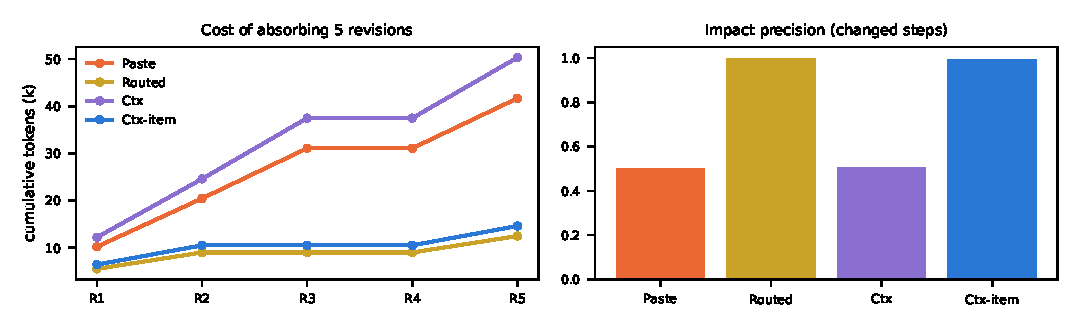
\includegraphics[width=0.95\linewidth]{context_cost.pdf}
\caption{Left: the running total cost of the five changes, by way of sharing. Right: how exactly each way marked
what to redo (explained in \Cref{sec:exact}).}
\label{fig:cost}
\end{figure}

\paragraph{Reading the numbers.}
\begin{itemize}[leftmargin=*]
\item \textbf{Item-level pinning versus paste.} About 2.8 times fewer tokens, and 2.8 times fewer AI calls (45
      against 124). This holds for every project and both models (between 2.1 and 3.2 times). The 95\% interval
      for the saving per project is 19 to 34 thousand tokens.
\item \textbf{Whole-notebook pinning is no better than paste.} It costs about 20\% \emph{more} than paste (50.3k
      against 41.7k tokens), because its prompts carry the extra labelled section and it redoes just as much. In
      R3, where an unneeded note is added, it redoes every job while item-level pinning redoes none. Pinning
      \emph{one note} is what saves the money; pinning the notebook does not.
\item \textbf{Item-level pinning versus routed paste: routed is cheaper.} Both make the same number of AI calls
      (about 44--45), but routed paste uses about 15\% fewer tokens (12.5k against 14.6k for the five changes; per
      project between 6\% and 34\% fewer), because its prompts do not carry the labelled notebook section.
      This is the one comparison where our proposal loses on cost, and we report it plainly.
\item \textbf{So why use it?} Routed paste is only cheap if a person keeps the routing table right, and the table
      is never checked by anything. The notebook works out ``who needs to redo what'' by comparing fingerprints,
      records who used which version, and fails safe when a note disappears. The extra price is about one sixth
      more tokens, with no extra AI calls. Our study measures that price; it does not measure how often a
      hand-kept table drifts out of date, which is a question about people that we did not test.
\item \textbf{The build costs a little more with the notebook} (12.6k with Ctx-item against 11.3k with routed
      paste), for the same reason.
\end{itemize}

\Cref{tab:models} splits the totals by model. The picture is the same for both.

\begin{table}[h]
\centering\small
\caption{Cost of the five changes per run by model (thousands of tokens, AI calls).}
\label{tab:models}
\begin{tabular}{@{}l r r r r@{}}
\toprule
 & Paste & Routed & Ctx (whole) & Ctx-item \\
\midrule
7B model (24 runs each) & 46.5k (138) & 13.7k (49) & 54.6k (137) & 15.7k (49) \\
27B model (8 runs each) & 27.4k (82) & 8.9k (30) & 37.5k (93) & 11.4k (32) \\
\bottomrule
\end{tabular}
\end{table}

\paragraph{Did the work stay as good?} We checked that the five fixed ``canary'' functions of each project keep
their exact required behaviour after the build and after the last change. In every one of the four ways, they all
did (100\%). That is reassuring, but it also means this check is \emph{saturated}: it cannot tell the four ways
apart, and it says nothing about harder quality. As in the earlier study, the generated code almost never passes
a project's full test suite with these models, so we do not claim the code is correct, only that the stated
constants survive.

\subsection{Did the system mark the right things?}\label{sec:exact}

Here we check the design against the plan. For every step we compare the set of jobs the system marked as
to-dos with the set that should have been redone.

\begin{table}[h]
\centering\small
\caption{How well each way marked what to redo, on steps where something should change (precision: how many marked
jobs were right; recall: how many right jobs were marked), and how often a step with nothing to change still made
AI calls.}
\label{tab:impact}
\begin{tabular}{@{}l r r r r@{}}
\toprule
 & Paste & Routed & Ctx (whole) & Ctx-item \\
\midrule
Precision & 0.50 & 1.00 & 0.50 & 0.99 \\
Recall & 1.00 & 1.00 & 0.97 & 0.97 \\
Steps with nothing to change that still redid work & 50\% & 0\% & 50\% & 0\% \\
\bottomrule
\end{tabular}
\end{table}

\textbf{How to read this table honestly.} The numbers for Paste and Routed are \emph{consequences of how those two
ways are defined}: paste redoes everything, so half of the jobs it redoes are unnecessary; a correct routing table
is exact by definition. They are not discoveries, and we do not draw conclusions from them. The informative row
is Ctx-item, where the system, not a person, makes the choice: it marked almost exactly the right jobs
(precision 0.99), and never redid work on a step where nothing should change. In 91\% of the steps in which no job
had failed validation earlier, the marked set was \emph{exactly} the right one. The remaining differences have one
cause: a job that failed its checks on an earlier change keeps an out-of-date fingerprint (so it counts as a
to-do), but its retry is cached as failed and costs no AI call; and a job that never got an accepted answer has
no fingerprint at all, which lowers recall.

\paragraph{Asking who used which note.} The lookup of \Cref{lst:influence} agreed with what the AI had actually
been shown, with precision 1.00 and recall 1.00, for both ways that use the notebook. This is a check that the
system's records match reality, not a measurement of how many influences exist.

\subsection{Does the logbook change anything?}

We tested this with a \emph{replay}. After a normal run, we ran the whole five-step schedule again, but this time
every AI prompt was answered from the first run's recording instead of calling the model. That removes random
variation, so any difference in the final result can only come from the logbook. We did this four ways: no logbook,
local logbook, logbook with Nostr, and Nostr with the relay switched off.

\begin{table}[h]
\centering\small
\caption{Replay results, 32 replays (one per project, model and seed).}
\label{tab:replay}
\begin{tabular}{@{}l r@{}}
\toprule
Check & Result \\
\midrule
Final state identical with Nostr attached & 100\% \\
Prompts sent identical with Nostr attached & 100\% \\
Final state identical with the relay down & 100\% \\
Prompts sent identical with the relay down & 100\% \\
Prompts missing from the recording (would count as a violation) & 0 \\
Events queued during an outage, on average & 703 \\
Outboxes that emptied completely after the relay returned & 100\% \\
Two machines ended with the same shared notebook & 100\% \\
\bottomrule
\end{tabular}
\end{table}

\paragraph{Is the logbook complete?} From the local logbook alone, every finished job's fingerprint and its pinned
note versions could be rebuilt: 100\%. From the signed Nostr copies alone, also 100\%, and all published events
passed signature checks. A caution: the engine writes these events itself, so this proves the events contain
\emph{enough} information, not that they are independent evidence.

\paragraph{What does it cost?} A run produces about 700 events (about 425 kilobytes). With the AI answers
replaced by instant recordings, which is the worst case for the relative cost, the local logbook adds
0.003 milliseconds per event (about 4\% of the engine's own time), and signing and queueing for Nostr adds about
0.2 milliseconds per event. Against AI calls that take seconds, this is not measurable.

\paragraph{Does it leak?} In standard mode we searched all events for the secret markers, generated code and
prompt text: zero occurrences. Notes of ``shareable'' contexts are the exception by design (they carry their
text across machines). This tested our markers; it does not rule out learning something from fingerprints, job
names or error messages.

\subsection{What happens when things break?}

We injected failures on purpose, in four families, into every run, and checked whether the system noticed.

\begin{table}[h]
\centering\small
\caption{Injected failures. 576 injections, 32 per kind. ``Noticed'' means the intended signal appeared (an event, an
error, a rejected message, a non-empty outbox).}
\label{tab:faults}
\begin{tabular}{@{}l p{8.2cm} r r@{}}
\toprule
Family & Failure injected & Noticed & Silent damage \\
\midrule
\multirow{2}{*}{Access to notes} & a reader is revoked; a context expires; a context is missing & 100\% & 0 \\
 & a non-writer writes; a forged author; two writers at once & 100\% & 0 \\
\midrule
The AI & its answer is rejected by the checks; the call itself fails & 100\% & 0 \\
\midrule
\multirow{2}{*}{Nostr messages} & bad signature; wrong key; unknown agent; wrong team; non-writer & 100\% & 0 \\
 & tampered contents; unknown context; forked version; duplicate delivery & 100\% & 0 \\
\midrule
Relay down & the relay is offline during a run & 100\% & 0 \\
\midrule
Control & an unrelated context changes (nothing should happen) & 100\% nothing & 0 \\
\bottomrule
\end{tabular}
\end{table}

All 576 injected failures were noticed, none ended in silent damage, and the harmless control correctly created no
work. When access was revoked, a context expired, or a context was missing, the first error event appeared 7
events into the run, and no prompt was ever sent without the notes it declared.

We want to be careful about what this shows. We chose the failures and we chose the signals that count as
noticing them, so this is a thorough test of the design, not an independent estimate of how often a real failure
would be caught.

\paragraph{Two failures it is built \emph{not} to catch.} We also added two probes of what the design cannot see.

\begin{enumerate}[leftmargin=*]
\item \textbf{Edit the instructions in the rule itself.} We changed the prompt text of a job's rule directly. The
      system created \emph{no} to-do in all 20 runs, because the fingerprint covers declared inputs and notes, not
      the rule's own prompt. If a rule author pastes knowledge into a rule instead of using the notebook, the
      system cannot see it. This is exactly the problem of Paste, and it is why we recommend putting knowledge in
      the notebook.
\item \textbf{A permitted writer publishes wrong or contradictory knowledge.} We had the Security Reviewer replace
      its finding with one that said the opposite. The system treated it as an ordinary revision: 8 to 22 jobs were
      marked as to-dos and redone, and nothing was flagged. The notebook controls \emph{who may write and which
      version was used}, not whether a note is \emph{true}.
\end{enumerate}

\takeaway{Every failure of access, signatures, versions, relay or AI that we injected was noticed; the two things
the design does not promise to catch, edits to the rule text and wrong-but-allowed notes, were not.}

\subsection{A sanity check against the earlier study}

Before the new experiments we re-ran the earlier study's change-propagation comparison on all eight projects with
the 7B model (one seed). The substrate behaves as it did before: the structured hand-offs kept all 40 of 40
canary functions, against 5 of 40 for free-text hand-offs and 0 of 40 for a shared schema, marked exactly the
right jobs after each change (precision and recall 1.00), and a change cost about 0.5 thousand tokens against
8.3 thousand for free text and 4.2 thousand for a shared schema. The same comparison with the 27B model was
only partly completed (5 projects, build step only, 25 of 25 canaries against 10 of 25 for free text), so we
do not report it as a result. This replicates the earlier study; it is not a contribution of the new work.

% ===========================================================================
\section{What it cannot do, and what we are unsure about}\label{sec:limits}
% ===========================================================================

\begin{itemize}[leftmargin=*]
\item \textbf{The test knowledge is artificial.} The two findings are instructions with a secret comment marker. That
      is good for knowing for certain whether knowledge arrived, but it does not show that knowledge improved the
      code, nor that stale knowledge causes real defects. A test where the knowledge changes behaviour (a required
      call, a forbidden pattern checked by a program) is the most important next step.
\item \textbf{There are only two findings and two kinds of consumers.} The savings over paste are bounded by that
      small number, and we expect them to grow with more findings and more consumers. We did not test that.
\item \textbf{Routed paste is the right comparison, and it is cheaper.} Our proposal is about 15\% more expensive
      in tokens at equal calls. What it adds is automation, a record of who used what, and fail-safe behaviour.
      Whether hand-kept routing tables really drift is a human question that we did not test.
\item \textbf{Few models and projects.} Eight Python projects and two open models from one family on one
      machine. The 27B model ran on four projects and two seeds. We make no claims about other models, other
      languages, or people working with agents.
\item \textbf{The quality check is saturated.} Every way kept all canaries, so the check cannot rank them.
\item \textbf{The logbook was tested by replay, not on a real network.} A replay removes sampling noise, but it
      does not test delays, partial delivery or a hostile relay. Those were simulated by injecting failures.
\item \textbf{Our fingerprints are shortened to 64 bits,} and the shortened fingerprints in the logbook are not
      secret: guessable text can be confirmed by trying guesses.
\item \textbf{Several writers per notebook are not guaranteed to agree.} Sharing is designed for one writer per
      context, with the first valid update winning.
\end{itemize}

\paragraph{Problems we found and fixed along the way.}
While preparing these experiments, review of the code turned up three real defects. (i)~When two valid updates for the
same version arrived at once, one could silently replace the other before being judged; they are now both
judged, with a test that fails without the fix. (ii)~In host mode the finished-answer event carried no pins, so
the notebook metrics read zero; it now carries them. (iii)~A results file leaked a file path; it is now
scrubbed. We also fixed that the experiment's random seed was only a label and was never sent to the model.

% ===========================================================================
\section{Try it yourself}\label{sec:try}
% ===========================================================================

All commands run from the repository root. The numbers in this document can be regenerated from the logs.

\begin{lstlisting}[style=raw, caption={Reproducing the results.}, label={lst:repro}]
python -m evaluation.harness.validate_references            # which projects qualify
python -m evaluation.harness.record_environment             # model and machine record
evaluation/results/follow-up-study/run_context_study.sh qwen2.5-coder:7b "1 2 3"
python -m evaluation.analysis.follow_up_aggregate --validate-legacy   # tables, figures, numbers
python -m evaluation.harness.chakin_context_walkthrough     # the listings in this document
python -m pytest tests/test_follow_up_context_study.py      # checks the experiment code itself
\end{lstlisting}

A \emph{safety note}: the checks of the prototype run AI-written code inside the experiment process. Run the
experiments in a container or a disposable folder.

% ===========================================================================
\section{Glossary}\label{sec:glossary}
% ===========================================================================

\begin{table}[h]
\centering\small
\begin{tabularx}{\textwidth}{@{}l X@{}}
\toprule
Term & Meaning \\
\midrule
Agent & An AI model playing one role (analyst, architect, developer, tester, reviewer). \\
Hand-off & The way one agent's work becomes input for the next, defined as a fixed transformation. \\
Job (binding) & One value an AI fills in, such as the body of one function, from a declared input. \\
Footprint & The pieces of input a job is allowed to see. \\
Stamp (fingerprint) & A short code summarising everything an AI was shown when a value was accepted. \\
Obligation (to-do) & A finished value whose current fingerprint no longer matches; it must be redone. \\
Context (notebook) & A shared collection of notes with versions and an access list. \\
Item (note) & One fact in a context, with an author and a type. \\
Pin & The record of which context, version and notes a finished job read. \\
Influence query & A lookup of which finished values read a given note. \\
Fail closed & If something needed is missing or not allowed, stop instead of guessing. \\
Event & One entry of the logbook: a typed record of something the team did. \\
Replay & Running the same schedule again, answering every prompt from a recording. \\
Nostr, relay & An open message format with signed messages, and a server that stores and forwards them. \\
Canary & A planted function whose required behaviour is an arbitrary constant, used to see whether instructions
survive a hand-off. \\
Seed & A number that fixes the model's random choices so a run can be repeated. \\
Token & The unit AI models read and are billed in; roughly a word fragment. \\
\bottomrule
\end{tabularx}
\end{table}

\paragraph{Where each number comes from.} All files are in \file{evaluation/results/follow-up-study/}.
\begin{itemize}[leftmargin=*,itemsep=1pt]
\item Delivery, churn, precision, recall: \file{csv/rq1\_traceability.csv}.
\item Cost: \file{csv/rq2\_cost\_summary.csv} and \file{csv/rq2\_cost\_per\_run.csv}.
\item Logbook checks: \file{csv/rq3\_observability.csv}.
\item Injected failures: \file{csv/rq3\_faults.csv} and \file{csv/rq3\_fault\_summary.csv}.
\item Projects that qualify: \file{csv/reference\_validity.csv}. Model and machine: \file{environment.json}.
\item Raw logs: the \file{raw/} folder, one JSON line per step.
\end{itemize}

\end{document}
